%
%  Introduction
%

\begin{section}{Particle Physics at the LHC}

Over the last century, the Standard Model (SM) has been shown to be the most accurate description of the fundamental construction and operation of the universe, but it is still incomplete, giving rise to many theories including Supersymmetry (SUSY), a popular extension of the Standard Model. It predicts a partner particle to every SM particle, which would resolve some particularly bothersome issues with the Standard Model like fixing the mass of the Higgs Boson, the identity of Dark Matter, and many others. Assuming SUSY is real, supersymmetric particles are expected to appear in high-energy collisions at the Large Hadron Collider (LHC). However, direct evidence for SUSY, or for any other competing theory, has yet to be discovered. Therefore, the pursuit of direct discoveries of new physics -- where ``new physics" is herearfter used to refer to evidence for Beyond Standard Model (BSM) particles -- is in a state of flux at the time of writing, and there is a growing doubt within the High Energy community that any discovery is likely to be made in the near future (i.e. within the next century). In response, CERN is investing in enhancing the LHC itself, first during a brief, two-year (2019 to 2021) shutdown period, then during a much longer overhaul for the High-Luminosity LHC (HL-LHC) with the hope that upgraded software and hardware and an enormous increase in data from the HL-LHC will push the field forward. In addition, contributions from the LHC may come from an analysis philosophy that does not fit the popular conception of scientific progress: rather than focusing on finding direct evidence of new physics, perhaps it is more useful to find new inconsistencies with the Standard Model to point future experiments in the right direction. This philosophy has always existed, and many such studies have been performed, but it has had understandably little recognition compared to achievements like the famous discovery of the Higgs boson. However, raising new, concerning questions is just as important as discovering their answers, since the former motivates the latter. In the context of experiments at the LHC, raising a concerning question is as simple as poking another hole in the Standard Model, but the question is only useful if it is more answerable than questions like a seventy-percent deficit in the current description of the makeup of the universe (dark matter) or the possibility of the quantization of gravity at energy scales beyond comprehension (gravitons). Nevertheless, there is a future worth watching at the LHC.

\end{section}

\begin{section}{The Compact Muon Solenoid}

The Compact Muon Solenoid (CMS) is a general purpose detector at the LHC, meaning it probes for the existence of a variety of new physics. The detector's namesake is a ``compact'' solenoid, the largest superconducting magnet ever built (with a length of 15m and diameter of 7m), that generates a 4T magnetic field strong enough to pull many high-energy, charged particles produced in a proton-proton collision towards CMS's detector layers\cite{CMS:1994hea}. Particles first encounter the tracker, which is composed of several layers of silicon pixels and strip detectors. Essentially, a through-going particle leaves a cascading charge deposit that can be measured as an electrical signal. This results in an accurate measurement of the particle's position as it passes through various sections of the tracker, which can then be reconstructed to give the particle's entire trajectory. Track information provides fundamental insights like the charge and momentum of a particle, for instance, which can be inferred from the curvature of the particle's trajectory. Having passed through the tracker, particles then encounter the calorimeters, which will measure the final energies of emergent particles when possible. Energies of particles that interact by the electromagnetic force, electrons and photons, are measured by the Electromagnetic Calorimeter (ECAL) while those that interact by the strong force, hadrons, are measured by the Hadronic Calorimeter (HCAL). Finally, particles that escape the ECAL and HCAL -- now only muons and weakly interacting particles -- encounter the muon layer, where muons are tracked further, before leaving the bounds of CMS. The presence of neutrinos, which mostly pass through the detector undisturbed, and possibly yet-undiscovered particles can only be inferred. Conservation of momentum is key here: invisible particles will show up as missing energy in comparing the sum of the measured particle momenta to the overall energy of the collision.

\begin{figure}[htb]
\begin{center}
\subfloat[Cutaway view of CMS detector.]      {
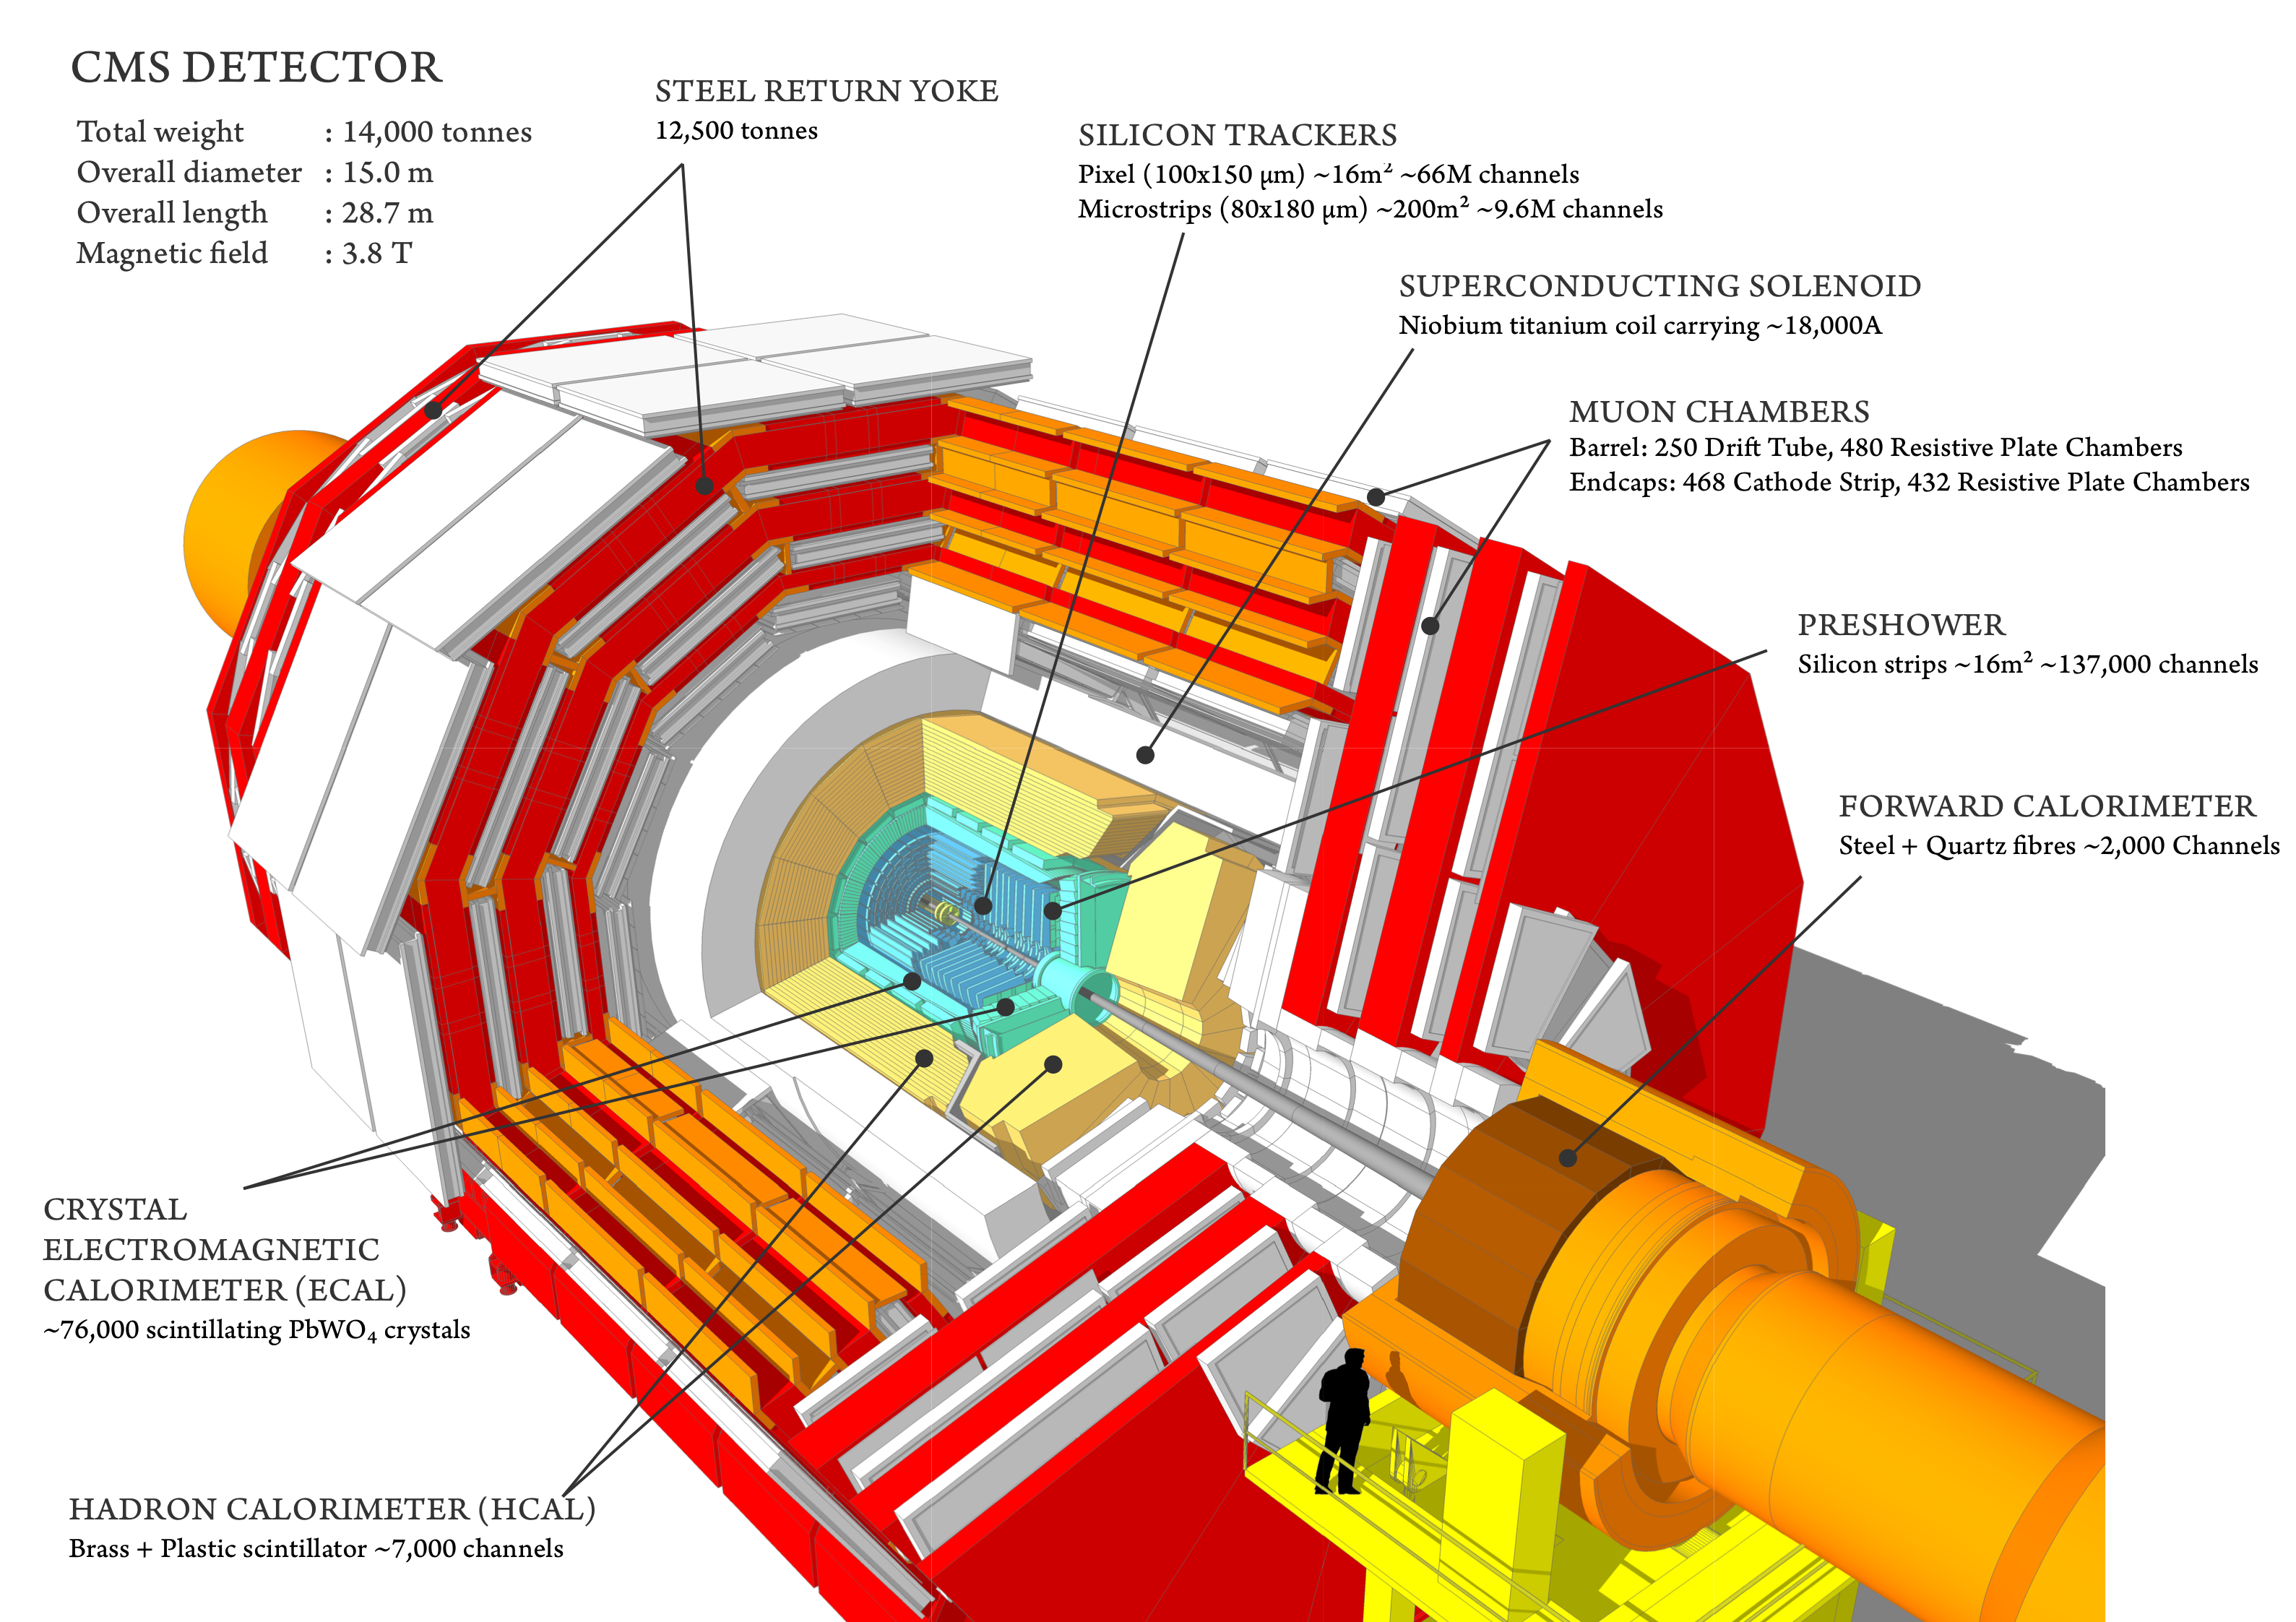
\includegraphics[width=.45\linewidth]{Dissertation/fig/cms-xsec.png}
}\quad
\subfloat[Illustration of detector layer response.]      {
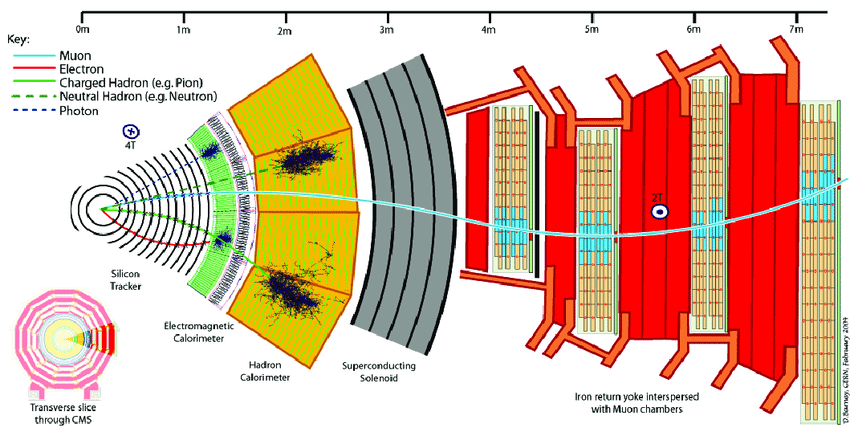
\includegraphics[width=.45\linewidth]{Dissertation/fig/cms-slice.png}
}
\end{center}
\caption{Visualizations of the design and function of CMS.}
\label{fig:cms-xsec}
\end{figure}

\end{section}